\documentclass[12pt, twoside]{article}
\usepackage[letterpaper, margin=1in, headsep=0.5in]{geometry}
\usepackage[english]{babel}
\usepackage[utf8]{inputenc}
\usepackage{amsmath}
\usepackage{amsfonts}
\usepackage{amssymb}
\usepackage{tikz}
\usetikzlibrary{quotes, angles}
\usepackage{graphicx}
\usepackage{enumitem}
\usepackage{multicol}
\usepackage{hyperref}

\newif\ifmeta
\metatrue %print standards and topics tags

\title{IB Mathematics}
\author{Chris Huson}
\date{January 2022}

\usepackage{fancyhdr}
\pagestyle{fancy}
\fancyhf{}
\renewcommand{\headrulewidth}{0pt} % disable the underline of the header
\raggedbottom


\fancyhead[LE]{\thepage}
\fancyhead[RO]{\thepage \\ Name: \hspace{4cm} \,\\}
\fancyhead[LO]{BECA / IB Math 03-Quadratic functions\\* 27 January 2022}

\begin{document}

\subsubsection*{4.4 Do Now Quiz: Cubic functions and graphing}
\begin{enumerate}
\item Shown in the plot below is the function $f(x)=-0.5x^{3}+x^{2}+5.5x-6$
\begin{enumerate}
    \item Write down the value of $f(0)$. On the graph, mark the point for $f(0)$ with a star.\vspace{1cm}
    \item Write down the solutions to $f(x)=0$. Mark them with ``X'' marks on the graph.\vspace{1cm}
    \item Mark the local maximum and minimum on the graph with their coordinates rounded to the nearest hundredth.
    \item Mark the portion of the function that is \emph{increasing} with a squiggly line.
\end{enumerate}
\begin{center}
    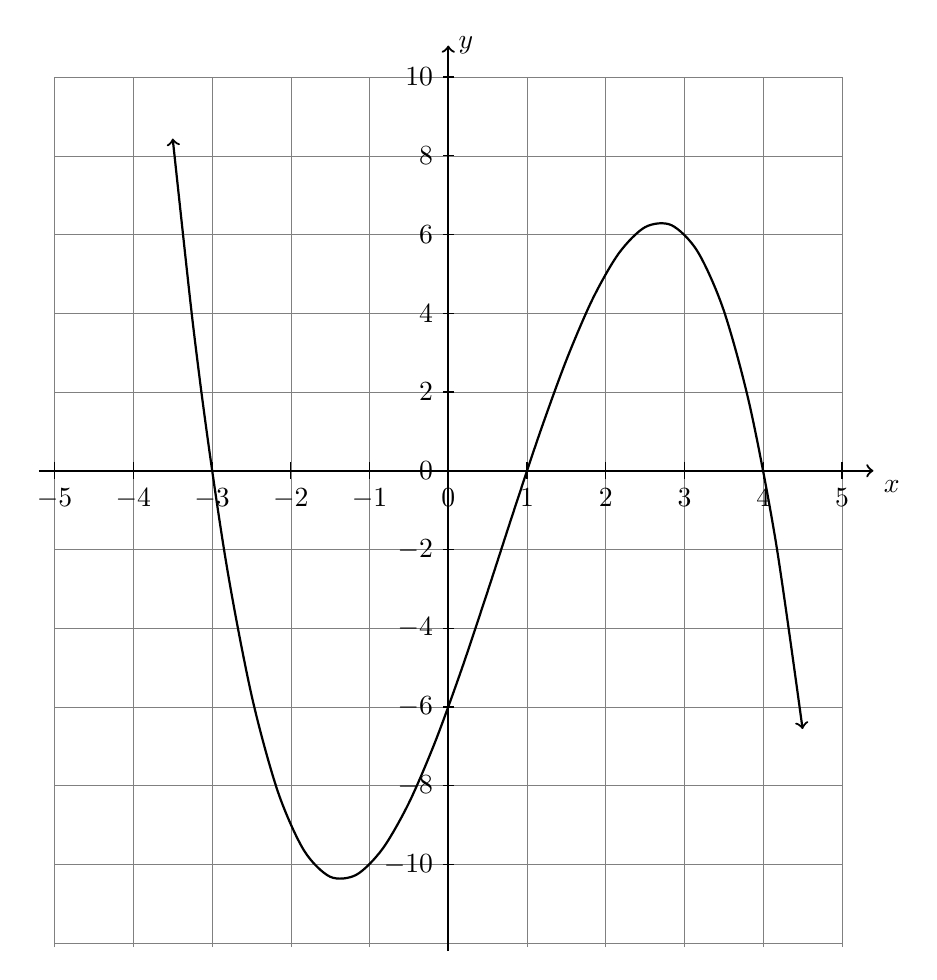
\begin{tikzpicture}[x=1cm, y=0.5cm, scale=1]
        \draw [help lines] (-5,-12.1) grid (5,10);
        \draw [thick, ->] (-5.2,0) -- (5.4,0) node [below right] {$x$};
        \draw [thick, ->] (0,-12.2)--(0,10.8) node [right] {$y$};
        \foreach \x in {-5,...,5}
            \draw[shift={(\x,0)}] (0,3pt)--(0,-3pt) node[below] {$\x$};
        \foreach \y in {-10,-8,-6,...,10}
            \draw[shift={(0,\y)}] (2pt,0pt)--(-2pt,0pt) node[left]  {$\y$};
        \draw [<->,thick,smooth,domain=-3.5:4.5] plot(\x,{-0.5*(\x)^3+(\x)^2+5.5*(\x)-6});
    \end{tikzpicture}
\end{center}

\newpage
\item Given the function $h(x)=x^3-2x^2-5x+6$.
    \begin{enumerate}
        \item Write down the $y$-intercept. Mark it on the plot.
        \item Show that $1$ is an $x$-intercept because $x=1$ is a solution to $f(x)=0$. Mark $(1, 0)$ on the graph as an $x$-intercept.\vspace{2cm}
        \item The other $x$-intercepts are $3$ and $-2$. Mark them on the plot.
    
        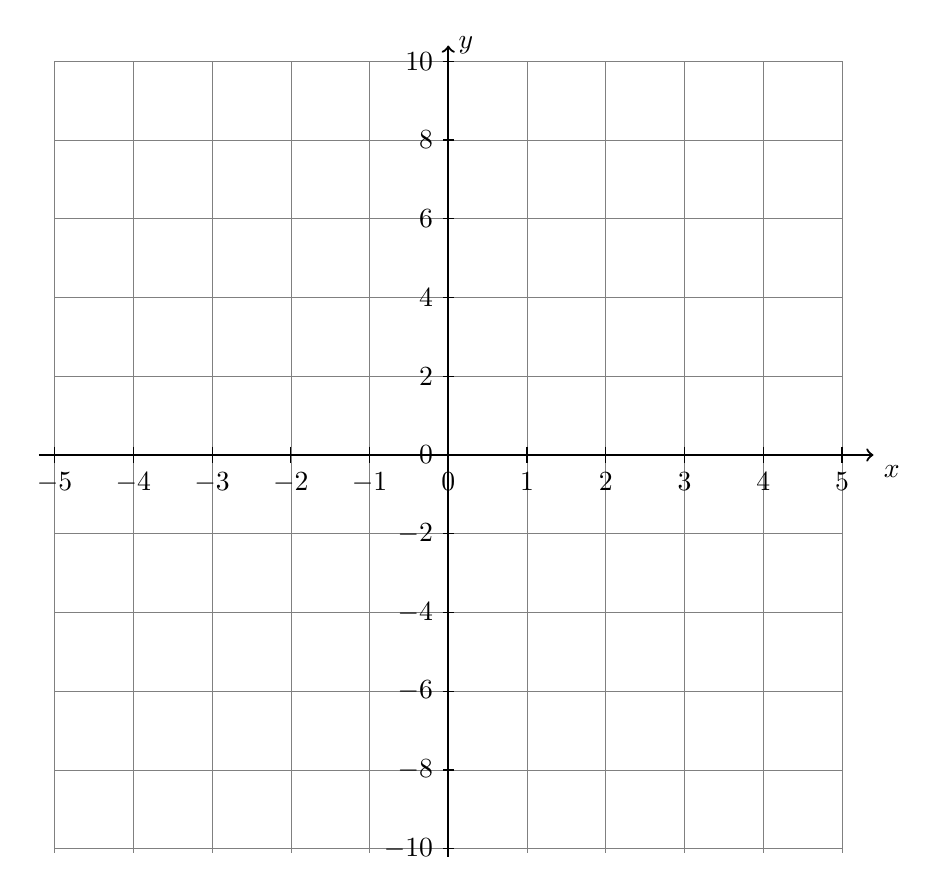
\begin{tikzpicture}[x=1cm, y=0.5cm]
            \draw [help lines] (-5,-10.1) grid (5,10);
            \draw [thick, ->] (-5.2,0) -- (5.4,0) node [below right] {$x$};
            \draw [thick, ->] (0,-10.2)--(0,10.4) node [right] {$y$};
            \foreach \x in {-5,...,5}
                \draw[shift={(\x,0)}] (0,3pt)--(0,-3pt) node[below] {$\x$};
            \foreach \y in {-10,-8,...,10}
                \draw[shift={(0,\y)}] (2pt,0pt)--(-2pt,0pt) node[left]  {$\y$};
            %\draw [<->,thick,smooth,domain=-2.5:3.5] plot(\x,{(\x)^3-2*(\x)^2-5*(\x)+6});
        \end{tikzpicture}
    
        \item Graph the function on a calculator or computer and, hence, sketch the curve.
    \end{enumerate}

\end{enumerate}
\end{document}



